%  Revised on Oct 24, 1999 (done on Aug 20)--spring.
%

%\documentstyle[12pt]{article}
\documentclass[12pt,a4paper]{article}

%\usepackage[square, comma, sort&compress]{natbib}
%\pagestyle{foot}
\textheight=255mm
\textwidth=175mm
\topmargin=-2.5cm
\oddsidemargin=-1cm
%\parskip 3mm
%\setcounter{page}{1}

\usepackage{ifsym}
\usepackage{cite}
\usepackage{amsmath}
\usepackage{amsfonts}
\usepackage{amssymb}
\usepackage{fancyhdr}
\usepackage{titlesec}
\usepackage{graphicx}

\pagestyle{fancy}
\fancyhead{} % 清除所有頁首設定
\fancyfoot{}
\renewcommand{\headrulewidth}{0pt}
\renewcommand{\footrulewidth}{0pt}
\setlength{\headwidth}{\textwidth}

\lfoot{表 C012}
\cfoot{共~~\pageref{LastPage}~~頁~~第{~~\thepage~~}頁}
\input{epsf}
\usepackage{epsf}
\usepackage{algorithm}%演算法要用到的
\usepackage[noend]{algorithmic}
\usepackage{setspace}
\usepackage{dsfont}
\usepackage[amsmath,thmmarks]{ntheorem}
\usepackage{indentfirst}               %使第一段文空格
\usepackage{multirow}                  %可使用兩排

\usepackage{fontspec}                    %加這個就可以設定字體 
\usepackage{xeCJK}                       %讓中英文字體分開設置 
%\usepackage[boldfont]{xeCJK}   %允許粗體和斜體
% ps. 使用粗體後, 編出來的pdf複製內文會便亂碼. 囧
\setCJKmainfont{標楷體}                   %設定中文字型 
\setmainfont{Times New Roman}            %設定主要字型,也就是英文字型 
\XeTeXlinebreaklocale "zh"               %這兩行一定要加,中文才能自動換行 
\XeTeXlinebreakskip = 0pt plus 1pt       %這兩行一定要加,中文才能自動換行

%以下非必要,但對於切換字型蠻好用的。
\defaultCJKfontfeatures{AutoFakeBold=5} %以後不用再設定粗斜 
\newCJKfontfamily\Kai{標楷體} %定義指令\Kai則切換成標楷體 
% \textbf{\Kai 這邊文字會變成標楷體粗體}}

\newcommand{\Fig}[1]{圖~\ref{#1}}
\newcommand{\Eq}[1]{方程式~(\ref{#1})}
\newcommand{\Tab}[1]{表~\ref{#1}}
\newcommand{\Chp}[1]{Chapter~\ref{#1}}
\newcommand{\Sec}[1]{Section~\ref{#1}}
\newcommand{\Chp}[1]{第~\ref{#1}~章}
\newcommand{\Sec}[1]{第~\ref{#1}~節}


% define a macro
%\def\texpsfig#1#2#3{\vbox{\kern #3\hbox{\special{psfile=#1}\kern #2}}\typeout{(#1)}}

\begin{document}
\newtheorem{thm}{Theorem}
\newtheorem{lem}{Lemma}
\newtheorem{cor}{Corollary}
\newtheorem{prop}{Proposition}
\newtheorem{conj}{Conjecture}
\input epsf   % load the epsf library

\baselineskip 7mm

\noindent
\textbf{\large 三、研究計畫內容 (以中文或英文撰寫)}
\begin{description}
\item[(一)]研究計畫之背景。請詳述本研究計畫所要探討或解決的問題、研究原創性、重要性、預期影響性及國內外有關本計畫之研究情況、重要參考文獻之評述等。如為連續性計畫應說明上年度研究進度。
\item[(二)]研究方法、進行步驟及執行進度。請分年列述:1.本計畫採用之研究方法與原因及其創新性。2.預計可能遭遇之困難及解決途徑。3.重要儀器之配合使用情形。4.如為須赴國外或大陸地區研究,請詳述其必要性以及預期效益等。
\item[(三)]預期完成之工作項目及成果。請分年列述:1.預期完成之工作項目。2.對於參與之工作人員,預期可獲之訓練。3.預期完成之研究成果(如實務應用績效、期刊論文、研討會論文、專書、技術報告、專利或技術移轉等質與量之預期成果)。4.學術研究、國家發展及其他應用方面預期之貢獻。
\item[(四)]整合型研究計畫說明。如為整合型研究計畫請就以上各點分別說明與其他子計畫之相關性。

\setlength\parindent{2em}    %設定每段落開始空兩格

%計數章節%%%%%%%%%%%%%%%%%%
\setcounter{section}{3}
\setcounter{subsection}{0}
%%%%%%%%%%%%%%%%%%%%%%%%%

\subsection{研究計畫之背景及目的}
\subsubsection{研究背景}%3.1.1
%%%%%%%%%%%%%%%%%%%%%%%%%
隨著各種形式的多媒體應用發展,對於網路頻寬的需求日益漸增,現在802.11 無線基地台已成為多數人不可或缺的生活工具,主要原因有三點,1、成本不高,大多數人都可負擔。2、架設簡單,不需要專人幫忙架設。3、傳輸速度快,足夠供給區域網路(LAN)內的使用者使用。綜合以上優點,WIFI在下世代網路是一個不可或缺的角色。所以如何在無線環境下將資料的吞吐量(throughput) 提升至理論最大值成了一門重要的課題。由於無線媒體是共享的,因此媒體存取控制(MAC)協定在協調媒體的存取以及效能最佳化的方面扮演著十分關鍵的角色。
此外[31]在802.11ax(WIFI6)中,CSMA/CA依舊是非常重要的媒體存取控制協議 (MAC protocol),當節點(node)有封包需要傳送時,會透過此機制判斷目前的通道是否可以傳輸,當偵測到的通道能量低於安全通道評估閾值(clear channel assessment CCA, threshold),則會再使用競爭視窗(contention window),透過隨機選擇初始後退計時器(backoff counter)來進行倒數,當節點偵測到空閒的通道時則計時器減1,但是若有傳輸在此通道進行時,則所有在同一個WLAN或其他WLANs的node計時器會暫停,直到計時器歸零時才能夠進行傳輸。
在CSMA/CA 架構中,多重速率、多點跳躍的無線網路環境之下,我們可以根據環境的變化,動態調整載波偵聽門檻(carrier-sensing threshold, Tcs ),並進一步平衡空間重複使用率(spatial reuse) 及傳輸可靠度(transmission reliability) 來達到整體網路效能(network capacity) 的最佳化。較低的Tcs 會使偵聽範圍(carrier-sensing range,dcs ) 擴大,此情況下能降低並行傳輸(concurrent transmissions) 造成的封包碰撞,進而提高資料傳輸的可靠度。然而,整體的網路效能(network capacity) 會因為節點對於資料傳輸的嘗試太過於保守而下降;反之,較高的Tcs 會使dcs 縮小,這樣一來空間重複利用率會得到顯著的提高,但相對的潛在訊號干擾亦會隨著增加,導致封包碰撞更頻繁的發生。因此於建立在CSMA/CA 基礎上的無線網路之下根據當下環境情況適當的調節Tcs 是非常重要的。在本計畫中,我們將提出一個於分散式的無線環境之下,在合理的計算時間內用以動態調節Tcs 之值的適應性機制,預期模擬結果將會證實我們所提出的演算法所求得的網路效能,相較於其他現有的載波偵聽調節相關演算法,可以表現得更為突出。\\



\subsubsection{研究目的}%3.1.2

在CSMA/CA 架構的無線環境中,以目前普遍使用的 IEEE 802.11 標準為例,實現了下列三個重要的機制: \\
1. 載波偵測(physical carrier sense):協調無線環境中各節點對媒體的存取,可偵測是否出現同步傳輸(simultaneous transmission)的情形及降低資料傳輸過程中所產生的干擾;\\
2. 二元指數後退演算法(binary exponential backoff algorithm):決定競爭視窗(contention window)的大小;\\
3. 支援多種資料傳輸率:根據封包傳送成功與否來調整資料傳輸速率(autorate function)。

載波偵測將決定節點是否能存取媒體。當一個節點在嘗試傳輸資料之前,會先對媒體進行傾聽,即環境中的電磁波信號強度。若該信號強度超過事先設定的載波偵聽門檻(carrier-sensing threshold, $T_{cs}$ ),表示媒體目前的情況為忙線(busy)而不進行資料傳輸。除了降低鄰近節點因雙向同步傳輸引起的碰撞之外,同時允許位在偵聽範圍(carrier-sensing range, $d_{cs}$ )外相對「安全」的節點在同一時間進行資料傳輸以提高空間重複使用率(spatial reuse)。雖然載波偵測概念簡單且實作效果佳,但已被\cite{sigcomm05_rwpcs}證實整體網路效能(network capacity)會因為不當選擇 $T_{cs}$ 值而下降。過低的 $T_{cs}$ 會使得環境中各節點顯得過於保守而喪失許多可能成功完成資料傳輸的時機,因而限制了其空間重複使用率。\cite{sigcomm05_rwpcs}的作者主張將載波偵測關閉以增進資料傳輸的效率,因此我們認為根據環境的變化來動態調節 $T_{cs}$ 的數值更為恰當。

當一個節點藉由載波偵測判定媒體目前的情況為閒置(idle)後,便會開始嘗試資料傳輸。判定資料傳輸成功與否的依據為「訊號/(干擾+雜訊)之比值」(Signal-to-Interference-and-Noise-Ratio, SINR)。若接收端感測到的 SINR 值低於最低門檻(SINR threshold, $\beta$),表示接收到的訊號無法被正確解讀導致傳輸失敗。造成資料傳輸失敗的原因有很多,如:若干個鄰近節點同時進行載波偵測且判定為閒置,導致各節點在同一時間存取媒體而發生碰撞;或是資料傳輸過程中被偵聽範圍($d_{cs}$)外的節點發出的訊號干擾,造成傳遞至接收端時 SINR 值過低,判定為傳送失敗;而二元指數後退演算法(binary exponential backoff algorithm)便因此被設計出用以解決競爭及碰撞的問題。

若接收端感測到的 SINR 值高於最低門檻 $\beta$,則視為傳輸成功,傳輸速率(data rate)的選擇將取決於 SINR 值的大小。隨著無線調變技術的進步,多重速率選擇已可應用於實作中,如 IEEE 802.11b 可選擇 4 種傳輸速率(1, 2, 5.5, 11 Mbps),IEEE 802.11a/g 可選擇 8 種傳輸速率(6, 9, 12, 18, 24, 36, 48, 54 Mbps),而IEEE 802.11n 同樣有 8 種傳輸速率可選擇(7.2, 14.4, 21.7, 28.9, 43.3, 57.8, 65, 72.2 Mbps)。IEEE 802.11ac依照頻寬不同有四種最大值(87.6, 200, 433.3, 866.7 Mbps), IEEE 802.11ax依照頻寬不同有四種最大值(143.4, 286.8, 600.5, 1201 Mbps)通常較高的 SINR 值能支援的較高的傳輸速率,為了進一步提高數據的吞吐量(throughput),當我們給定一 SINR 值,大多會選擇該值能承受的最大傳輸速率。\cite{mobicom01_ramp}的作者認為傳輸速率的調節是建立在預期接收端的通道品質的基礎上,因此提出了一個被稱為「Receiver-Based Auto-Rate mechanism, RBAR」的適應性速率調節 MAC 協定。如名稱所示,預期的接收端必須事先計算其通道品質並將其資訊回送至傳送端,傳送端再根據其資訊選擇最大可擔負的傳輸速率。 

SINR 值對於資料傳輸的成功與否,以及在複雜的無線環境之下能夠承受多大的傳輸速率,扮演著十分關鍵的角色。這些因素會更進一步地影響整體的網路效能(network capacity),而 SINR 值的大小與 $T_{cs}$ 的選擇息息相關。理論上較大的 $T_{cs}$ 值能夠提高空間利用率(spatial reuse),但由於 $d_{cs}$ 範圍外的節點所造成的干擾亦會令整體通訊品質下降而導致因為 SINR 值的降低必須退而求其次去選擇較低的傳輸速率,也因此在空間利用率與傳輸速率之間必須做出適當的取捨,才能夠進一步提升整體的數據吞吐量。 

我們透過延伸 Cali’s  model\cite{tn00_cali},將最終的網路效能(network capacity)表示成一由 $T_{cs}$, SINR, $\beta$ 與其他 PHY/MAC 的系統參數所組成的方程式,並經由調節 $T_{cs}$ 及競爭視窗(contention window)來觀察其結果,可得知網路吞吐量(network capacity)並不是單純的與 $T_{cs}$ 成正比或反比的關係。在不同的環境下調節 $T_{cs}$ 並計算當下的網路效能(network capacity),結果呈現出極為不規則的變動,因此無法藉此看出其規律。然而,現實情況下無線環境常隨著時間不斷地在改變,一些重要參數如節點個數、節點間距離等變化亦十分頻繁,而給定一組參數以計算出所有 $T_{cs}$ 對應的網路效能往往需耗費大量時間,導致計算出的結果已經不適用於目前的環境。 

因此,在變化快速的無線環境下,如何用最短的時間找出能夠提高網路效能(network capacity)並進一步找出理論最大值所對應的 $T_{cs}$ 將成為本計畫探討的議題。\\

%%(四)開始
\subsection{研究方法與執行進度}
\subsubsection{第一年研究方法與執行進度}

\begin{enumerate}
\setlength\parindent{2em}    %設定每段落開始空兩格
%-----------------------------------------------------------
\item [\bf A.]{\textbf{\Kai 利用調節載波偵聽門檻($T_{cs}$)實現空間多樣性 }}\\
\vspace{-2mm}

網路環境的空間重複利用率(spatial reuse),可以透過調整傳輸功率與載波偵聽門檻來決定,前者為各節點傳送資料時所使用的傳輸功率,後者則用來判定媒體是否處於閒置(idle)狀態的臨界值參數。此組參數將決定了網路環境的空間多樣性(spatial diversity),並且更進一步的影響其通道多樣性(channel diversity)。一些現有的研究,如:\cite{ccr2004_rws}、\cite{mobicom04_ssch}、\cite{mobihoc04_mcmac},裡面說明了關於實現通道多樣性的方法。

為了達到藉由調節 $T_{cs}$ 增進空間重複利用率的目的,\cite{vtc03_sr}、[17-19]透過估算及實驗結果來分析 $T_{cs}$ 對於整體網路效能(network capacity)的影響。 
\cite{vtc03_sr}的作者探討了節點較為密集的無線隨意網路(wireless ad hoc network)的空間重複利用率,無線電波的傳播與干擾所使用的模組是建立在通道訊號衰減(衰減參數 $\gamma$)及 SINR值上。在直線與 2-D 平面網路中利用這些參數來決定任兩個並行傳輸的節點(concurrent transmitter)之間的最短距離,以藉此實現最佳化的空間重複利用率。 

然而,MAC-layer 的標頭在計算空間重複利用率上是被忽略不計的,因此\cite{icc04_zhu}的作者以完美 MAC 環境為前提,基於\cite{vtc03_sr}的方法,提出一個改良型的載波偵測機制,透過給定接收端的功率、資料傳輸速率及網路拓樸模型,分別在直線與 2-D 平面網路下,來計算可最佳化整體資料吞吐量與空間多樣性的 $T_{cs}$ 值。 

在近期相關研究中,\cite{infocom06_zhai}展示了一個利用傳輸距離的變化、接收端對於信號敏感程度的差異及多點跳躍傳播的效應,來最佳化空間重複利用率的方法,並進一步歸納出「單一 $T_{cs}$ 值可適用於任意通道傳輸速率」的結論。此處我們假設:(1)所有接收端對信號敏感程度一致;(2)資料傳輸距離皆相同。由於載波偵聽門檻($T_{cs}$)會影響偵聽範圍($d_{cs}$),可探討不同 $d_{cs}$ 值對於通道傳輸速率的影響。如:給定一組載波偵聽數值並仔細觀察當下的網路情況,能夠推論出當時可實現的最大資料傳輸率。換句話說,不一樣的 $T_{cs}$ 值呈現出的最佳資料傳輸速率亦不同。 

\cite{infocom05_yang}的作者認為 MAC 標頭對於 $T_{cs}$ 的選擇具有十分顯著的影響,因此提出了一個將 MAC 標頭列為重要參數並用來計算無線隨意網路的整體吞吐量的分析模型,其定義了兩種型態的 MAC 標頭: (1) Bandwidth-independent (PLCP preamble and header, DIFS, SIFS) (2) Bandwidth-dependent (channel-rate-dependent data frame time) 。並進一步主張使用較小的 $d_{cs}$ 來提高同步傳輸(concurrent transmission)的數量。但其只考慮 1st-tier 內的節點所造成的干擾,而在\cite{vtc03_sr}中已證明此方法在節點分布較為密集的網路中效果有限,而我們所提出的分析模型會統計所有由 $d_{cs}$ 範圍外的同步傳輸所造成的干擾總和。此外,\cite{vtc03_sr}、[17-19]並未將 $T_{cs}$ 及資料傳輸速率做連結,而我們將針對不同的 $T_{cs}$ ,估算 $T_{cs}$ 範圍外的干擾程度來設定其最適合的資料傳輸速率。在「$d_{cs}$ 範圍內的同步傳輸(simultaneous transmission)必定會產生碰撞」方面,我們認為可藉由給定適當的資料傳輸速率 $r_i$ 使接收端所收到的干擾訊號不逾越 $P_r/\beta[i]$ 來避免碰撞的發生。($P_r$:接收端收到的訊號強度;$\beta[i]$:對於資料傳輸速率 $r_i$ 而言的最低 SINR 門檻值)。\\



%-----------------------------------------------------------
\item [\bf B.]{\textbf{\Kai 利用調節資料傳輸功率($P_{tx}$)實現空間多樣性 }}\\
\vspace{-2mm}

為了讓網卡傳輸功率受限的行動裝置實現降低訊號干擾與節能的目的,[12-14]提出了數個適用於單通道無線環境的演算法,這些演算法決定了在當下的環境中各個節點適用的最小傳輸功率;另一方面,[5]的作者展示了一個實例,說明功率控制不一定能夠有效的降低訊號干擾。此外,給定「訊號干擾」較為明確的定義後,進一步驗證拓樸控制(topology control)相關演算法,發現其對於降低訊號干擾並沒有較為顯著的貢獻。\cite{acm2005_smcwd}的作者提出了建立在分布密集的數十個 Wi-Fi 熱點(access point, AP)的無線區域網路上的功率控制及適應性速率調節演算法,主要目的為透過協調各 AP 的活動以降低傳輸功率的消耗,使整體系統維持合理的資料吞吐量(throughput)。此外,基於實際生活中對大規模資料流量的追蹤與觀察的基礎上,\cite{acm2005_smcwd}的作者做出了下列結論:透過對環境的適應並自動調節 AP 之間傳輸功率與速率,我們可以達成提升整體網路效能的目標。 然而,在本計畫所研究的分析模型中,我們假設所有節點使用相同的傳輸功率並調節 $T_{cs}$ ,另外以接收到的 SINR 值為基礎動態的決定每次資料傳輸所使用的傳輸速率。如\cite{mobicom06_kim}所述,給定的資料傳輸速率仍需符合 Shannon capacity 的限制,而空間重複利用率僅取決於傳輸功率與 $T_{cs}$ 的比值,這說明了調節傳輸功率和調節 $T_{cs}$ 的所產生的效應大致是相同的。 \\


%-----------------------------------------------------------
\item [\bf C.]{\textbf{\Kai 其他相關研究 }}\\
\vspace{-2mm}

近年來有各式各樣關於 $T_{cs}$ 、傳輸功率和其他 MAC 的相關參數對網路效能(network capacity)所產生的影響之研究。\cite{cst14_survey}便對這方面的研究做了一定程度的蒐集和統整,從中我們可以發現許許多多的作者對於如何適當的調節、運用這些參數都有著其獨特的見解。如\cite{adhoc11_park}、\cite{tmc08_hou}、\cite{tvt09_power}便是進一步的將 $T_{cs}$ 和傳輸功率做比較分析。\cite{adhoc11_park}]主張分開討論同質(homogenous)與異質(nonhomogenous)性網路下 $T_{cs}$ 與傳輸功率對網路效能的影響。在同質性網路下,透過數學推導於節點密度固定的情況之下將最佳 $d_{cs}$ 以一個由傳輸功率及 $T_{cs}$ 的方程式表示;而異質(nonhomogenous)性網路下,各個節點若各自獨立調整 $T_{cs}$ 將會導致網路效能不佳。\cite{tvt09_power}運用其設計的模組證明傳輸功率及 $T_{cs}$ 的選擇對於無線環境中網路效能的好壞有著很大的影響,其中 $T_{cs}$ 的重要程度又略大於傳輸功率,一旦選擇了適當的 $T_{cs}$ ,傳輸功率的調節對減少碰撞以提高網路效能相較於使用RTS/CTS 更有效果。而\cite{tmc08_hou}則是與\cite{tvt09_power}抱持著相反的主張,認為傳輸功率對網路效能的影響比 $T_{cs}$ 還要來得大,因此提出了一個用以調節傳輸功率及速率的分散式演算法,並進一步證明其較現有的 $T_{cs}$ 調節方法還來得有效率。 

以上的研究探討的內容大多集中於 $T_{cs}$ 和傳輸功率分析比較,但事實上競爭視窗(contention window, $CW$)和傳輸速率的設置對於網路效能的影響並不亞於$T_{cs}$ 和傳輸功率。如\cite{infocom08_zeng}便是在 IEEE 802.11 DCF 的環境下針對 $CW$ 進行較深入的綜合分析,並以由 Cali’s model \cite{tn00_cali}延伸的模組證明 $T_{cs}$ 和 $CW$ 的選擇對網路效能確實存在著一定程度的影響;\cite{infocom07_interplay}則更進一步的加入了多重傳輸速率(multi-rate)分析,即結合 $T_{cs}$ 、$CW$ 和傳輸速率這三者重要性相當可觀的參數去比較是否適當的調節這些參數對整體網路效能的影響程度。 

然而,上述所提到的相關研究都是在靜態的環境之下進行參數分析比較,沒有充分考量到現實環境所遭遇到的情形。例如\cite{infocom07_interplay}展示了節點個數為 10、62、200(分別代表鬆散、平均、密集)的環境之下由不同的 $T_{cs}$ 、$CW$ 和傳輸速率所輸出的網路效能(network capacity),其說明了在不同的環境之下 $T_{cs}$ 、$CW$ 和傳輸速率三者的最佳參數組合亦不同,這是假設其他參數(傳輸功率、節點間距離等)相同的情況之下,而現實中這些環境參數如:節點個數不可能完全靜止不變。因此,如何在有限的時間內根據當下環境「即時更新」(On-line adjusting)各項參數至最適當之值便成為了非常重要的課題。 

\cite{cccn08_phycs}、\cite{tmc09_aphycs,ton09_optwmn,infocom07_optcs,icl13_iter}各自提出數個動態調節 $T_{cs}$ 的適應性演算法。其中\cite{cccn08_phycs} 與\cite{infocom07_optcs}是以現有的參數值透過各自設計的演算法來預測當下環境可能的最佳 $T_{cs}$ 之值,但環境中節點並未彼此互相交換資訊而是採取類似「各自為政」的方式,即每個節點獨立進行參數的調整。但可能會衍生出一些問題,如某些節點在調節參數的時候可能透過疑似作弊(cheating)的手段以取得較多的網路資源,另外在不斷變化的環境之下常常會因為預測出現誤差而導致網路效能不甚理想。\cite{icl13_iter}則是透過數值分析的方式來計算最佳 $T_{cs}$ 之值,但其目標在於提升頻譜效率(Area Spectral Efficiency, ASE),然而高 ASE 僅表示在同樣的頻寬之下傳送的資料量較大,類似採用高傳輸速率(如 48、54Mbps),但並不代表能夠獲得較高的整體網路效能(network capacity),原文中也未對網路效能進行模擬分析。而\cite{tmc09_aphycs}與\cite{ton09_optwmn}是以實際運作時的封包遺失率(Packet Error Rate, PER)來做為調整 $T_{cs}$ 的依據,其主張 PER 在特定範圍下能夠最大程度的提高網路效能,若 PER 過大即 $T_{cs}$ 過大,以至於各節點嘗試傳輸資料過於積極而導致碰撞頻繁發生,因此藉由降低 $T_{cs}$ 來緩和此現象以減少碰撞進而提高整體網路效能;相對的,PER 過小即為空間重複利用率(spatial reuse)過低而導致各節點嘗試存取媒體過於保守,同樣的藉由提高 $T_{cs}$ 來增加節點嘗試傳輸資料的頻率。

然而,上述\cite{cccn08_phycs} 、[27-30]所闡述之方法沒有考慮到競爭視窗 $CW$ 和傳輸速率對於網路效能的影響。這些演算法大部分是針對 $T_{cs}$ 做調節,對於適當的 $T_{cs}$ 值,如果選擇不當的 $CW$ 與傳輸速率,仍然會導致網路效能不佳。換句話說,如果欲更進一步的提升網路效能,根據環境適當的選擇 $T_{cs}$ 、$CW$ 及傳輸速率這個參數組合是非常重要且缺一不可的。很少演算法能夠同時對 $T_{cs}$ 、$CW$ 及傳輸速率這些參數做適應性調節。雖然\cite{ton09_optwmn}所提出的方法有包含 $T_{cs}$ 、$CW$ 及傳輸速率的調節,但其本身用意並不在於此且效能並不理想。\cite{tmc09_aphycs}跟大部分演算法一樣,僅針對 $T_{cs}$ 做調節,其方法類似\cite{ton09_optwmn}皆以 PER 為 $T_{cs}$ 搜尋的基礎。我們未來將詳細研究\cite{tmc09_aphycs}與\cite{ton09_optwmn}所提出的方法,在效能評估的時候,將做為我們比較與討論的對象。 \\

\item [\bf D.]{\textbf{\Kai 建立網路模型 }}\\
\vspace{-2mm}

考慮一個 IEEE 802.11 Distributed Coordination Function (DCF)為基礎下的多點跳躍、多重速率的無線網路環境,當一個節點欲傳送封包時會先對媒體傾聽以確認其目前的狀態,若判定為忙線(busy)則不會進行封包的傳送;反之,若持續傾聽了一段特定時間(被稱為 Distributed Inter-Frame Spacing, DIFS)而媒體狀態皆為閒置(idle),則接下來該節點會選擇一個 $0$ 到 $CW-1$ 的數值作為倒數計時器($CW$ 為目前設定的 contention window大小),當計時器倒數完畢時便會開始嘗試傳送資料。若封包被正確無誤的接收,接收端在一段特定時間後(被稱為 Short Inter-Frame Spacing, SIFS, 較 DIFS 短)會回傳一個ACK 封包告知傳送端封包已被成功接收;若封包傳送至接收端時發生碰撞,或是傳送端未能成功接收 ACK,則視為傳送失敗,此時傳送端會將 CW 值加倍,並重新安排該筆資料的傳輸直到重試次數達到上限。而 CW 設定值由最小值 $CW_{min}$ 開始,一旦發生傳送失敗便加倍,直到最大值 $CW_{max}$ 為止。 

在現實環境中,電磁波訊號會因為許多原因導致衰減,如通道衰減(傳播距離太長)、多重路徑衰減(訊號經過反射造成延遲)和遮影效應(受障礙物遮蔽),如\cite{book2002_wc}所言。然而,在本計畫中,我們將專注在由通道引起的訊號衰減,相關參數定義為: $P$ 為網路中各節點的傳輸功率、$D$ 為傳送端與接收端之間的距離、$G$ 為天線增益常數、$\alpha$ 為通道衰減參數(其值大約在2到4之間),接收端所收到的訊號功率 $P_r$ 為 $P_r = \frac{GP}{D^ \alpha}$。 我們假設距離 $D$ 值很小,使接收端在不用顧慮訊號干擾,能夠支援最大的資料傳輸速率。 

如\cite{sigcomm05_rwpcs}所述,有很多的方法能在實際的裝置上操作載波偵聽,而我們採用其中最普遍的方法:能量偵測。在嘗試傳輸資料之前,傳送端先偵測環境中的訊號強度,並與事先選定的 $T_{cs}$ 值比較。若偵測到的訊號強度大於 $T_{cs}$ 值則判定媒體目前的情況為忙線(busy),反之則為閒置(idle)。此外,由(3.1)式,我們定義載波偵聽範圍($d_{cs}$)為 $d_{cs} =  \big( \frac{GP}{T_{cs}} \big)^{ \frac{1}{\alpha}}$ 。此處我們定義 $d_{pg}$ 為無線訊號能夠傳播的最遠距離。 

當傳送端(tr)傳送封包給接收端(rcv)時,若此時另一個傳送端 t' (concurrent transmitter)恰好處在 tr 的 $d_{cs}$ 範圍外,並同時傳送封包給同一個接收端(rcv),將造成兩個傳送端的訊號在接收端 rcv 重疊,我們稱之並行傳輸(concurrent transmission)。而 tr 所發出的封包是否能被 rcv正確無誤的接收,取決於其 SINR 值是否高於其最低門檻(SINR threshold)。針對不同的資料傳輸速率 r[i],有不同的的 SINR 最低門檻 $\beta[i]$需求。若 rcv 在資料傳輸速率為 r[i]的情形下接收到的訊號的 SINR 值大於$\beta[i]$,表示訊號可被 rcv 成功解讀及 r[i] 可支援當下的網路環境。此處d(t',rcv)代表 t' 與 rcv 之間的距離。 
$$
SINR =  \frac{\frac{P}{D^ \alpha}}{ \sum_{t' \neq tr} \frac{P_{t'}}{d(t',rcv)^ \alpha} } \geq \beta[i]
$$
在無線環境中,除了由 $d_{cs}$ 外的節點所造成的訊號干擾之外,還有另一種被稱作同步傳輸(simultaneous transmission)的干擾源,即多個在 $d_{cs}$ 範圍內的傳送端在短時間同時偵測到媒體為閒置並同時進行資料的傳輸,此種干擾所造成的碰撞無法使用載波偵聽來避免。 

六角干擾模型(Hexagon interference model)常被用來計算在最糟的情況下的 SINR 值,即一定範圍內所有的節點同時對媒體傾聽並傳送封包。\Fig{fig:hexagon_model}說明了在接收端所處的最糟環境下所產生的干擾情形,根據 $T_{cs}$ 的定義,相鄰兩組並行傳輸(concurrent transmission)的最短距離為 $d_{cs}$ ,而 1st tier 干擾是由最靠近傳送端 tr 的六個節點($H_1 - H_6$)所引起,且\cite{tvt1986_cmrs}已證明了當接收端 rcv 與上述六個節點距離為 $d_{cs}-D$, $d_{cs}-D$, $d_{cs}-2/D$, $d_{cs}$ , $d_{cs}+2/D$, $d_{cs}+D$ 時受到干擾程度為最大(即 SINR 值最小)。而對接收端 rcv 而言,$H_1 - H_6$ 與在 $d_{cs}$ 範圍之外、$d_{pg}$ 範圍之內的節點都有可能成為訊號的干擾源,因此資料傳輸的成功與否及可用的傳輸速率大小將取決於整體訊號干擾的程度。

%-------------------
\begin{figure}[hbt]
\begin{center}
\centering {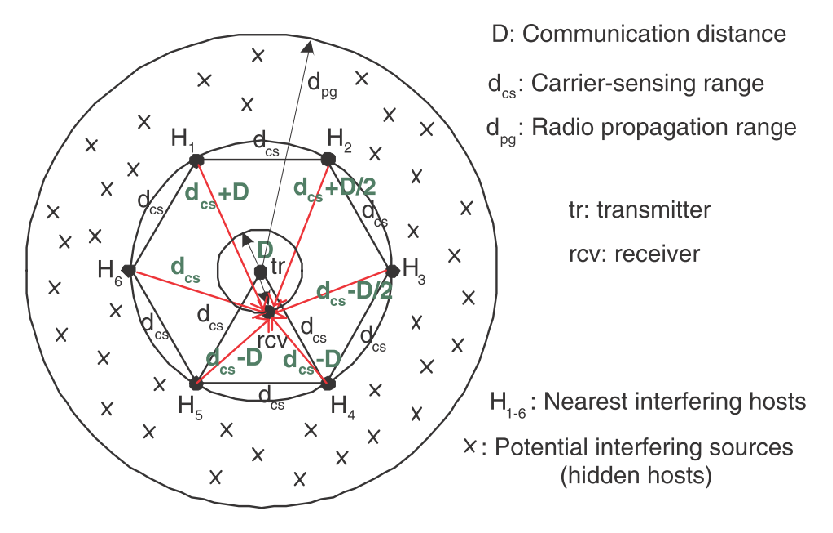
\includegraphics[width=8cm]{eps/hexagon_model.eps}}
\caption{六角干擾模型(Hexagon interference model)示意圖} \label{fig:hexagon_model}
\vspace{-0.2cm}
\end{center}
\end{figure}
%-------------------

在第一年的規畫裡,我們會先著手進行無線網路的相關研究,如:如何利用利用調節載波偵聽門檻($T_{cs}$)實現空間多樣性,利用調節資料傳輸功率($P_{tx}$)實現空間多樣性,探討相關研究,最後則是建立網路模型。建立完網路模型之後,我們可以深入分析造成干擾的因素並建立模型,接著推導網路效能方程式,尋找適當的參數使得整體網路效能(throughput)可以更為提升。\\


\end{enumerate}
\subsubsection{第二年研究方法與執行進度}

\begin{enumerate}
\setlength\parindent{2em}    %設定每段落開始空兩格
%-----------------------------------------------------------
\item [\bf A.]{\textbf{\Kai 結合傳輸功率選定及 $T_{cs}$調節的演算法(LMST-DCUA) }}\\
\vspace{-2mm}

作者\cite{tmc09_aphycs}提出一個結合傳輸功率選定(LMST)及 $T_{cs}$ 調節(DCUA)的演算法。其中 LMST為決定節點傳輸功率的演算法,其流程又分為資訊蒐集、拓樸(topology)建立及選定傳輸功率三個階段。在資料蒐集的階段,節點間藉由 Hello message 來交換彼此的資訊,如:節點編號、所在位置等。接著以 Prim's algorithm 建立包含鄰近節點資訊的最小成本擴張樹,最後再根據這些資訊來決定傳輸功率之值。而 DCUA 為該演算法的重點,全名為 Distributed carrier sense update algorithm,其概念為觀察資料傳輸過程中發生碰撞的頻率,進而調整載波偵聽門檻。流程如下: 
(1) 各節點分別各自計算其資料傳輸發生碰撞的機率(collision probability, $q_i$ ),即 $q_i = N_c / N_t$ ($N_c$ :發生碰撞的次數;$N_t$ :嘗試傳送資料的次數)。 
(2) 令一參數 $q_{i}th$ 為碰撞發生門檻,以決定每次資料傳輸後載波偵聽門檻(carrier-sense threshold, $x_i$ )的調節。 
(3) 每個 round 結束後將統計並計算出的 $q_i$ 值帶入演算法來決定這一個 round 所使用的 $x_i$ 值,其中 $\lambda_i$ 與 $v_i$ 為控制調節幅度大小的 step size 和權重參數。 

此演算法引入了空間重複利用率(spatial reuse)的概念,意即高門檻會形成低敏感度的環境,各節點嘗試資料的傳輸會較為踴躍,但較容易造成碰撞,因此當碰撞發生過於頻繁時須將門檻調低;而低門檻會形成高敏感度的環境,較能有效避免碰撞的發生,但相對的各節點在資料傳輸的方面也較為保守,易造成整體網路效能(network capacity)下降,出現此情形時便將門檻調高以增進整體網路效能。\\

%-----------------------
% 插入 algo 1
%-----------------------

\item [\bf B.]{\textbf{\Kai 結合傳輸速率選定與 $T_{cs}$ 調節的演算法(PCSadapt) }}\\
\vspace{-2mm}

全名為 PCS Adaptation Algorithm Based on Loss Differentiation \cite{ton09_optwmn},本身為一個結合傳輸速率選定與 $T_{cs}$ 調節的演算法,它將整個資料傳輸的流程分為 (1) adaptation ,(2) normal operation 兩個階段。

當處於階段(1)時,首先會進行傳輸速率的選定,環境中所有節點各自將其最小競爭視窗($CW_{min}$)設定為一較大的值,以避免碰撞頻繁發生。接著透過蒐集各節點的 RSSI (Received Signal Strength Indicator,一個類似 SINR、用來衡量接收端訊號強度的基準),RSSI 值小表示干擾或訊號衰減程度大,選擇低傳輸速率較為合適,相對的 RSSI 值大表示該節點可負荷較高的傳輸速率。實際操作時會先訂定一組「衡量標準」,如:$P_1, P_2, ..., P_M$ ,當 RSSI 值落在 $P_1$ 與 $P_2$ 之間選擇傳輸速率 $r_1$,落在 $P_2$ 與 $P_3$ 之間則選擇傳輸速率 $r_2$ ,依此類推,當所有節點選定傳輸速率後直到階段(2)結束之前都不會再更動。而傳輸速率選定後各節點便會進行數個 round 的資料傳輸,同時記錄 PER(Packet Error Rate),即傳輸失敗的封包數量及封包總傳輸數量之比值。每當一個 round 結束,其中一個被設定為 AP 的節點會蒐集所有節點所記錄的 PER 值,並選出最大者做為調整 $T_{cs}$ 的依據,詳細見\cite{ton09_optwmn}的演算法。
當所有的 round 結束之後,便會進入階段(2),所有節點將其 $CW_{min}$ 調回正常值並繼續資料的傳輸。在此階段表示參數調節完畢,將不會更動包含 $T_{cs}$ 在內的任何參數,每隔一段指定時間就會重新進入階段(1),再根據目前當下的環境資訊進行參數的調整。 

%-------------------
\begin{figure}[hbt] 
\begin{center}
\centering {\includegraphics[width=8cm]{eps/PCSadapt.eps}}
\caption{PCSadapt之運作流程示意圖} \label{fig:PCSadapt}
\vspace{-0.2cm}
\end{center}
\end{figure}
%-------------------


%-----------------------
% 插入 algo 2?
%-----------------------

\item [\bf C.]{\textbf{\Kai 網路效能方程式推導 }}\\
\vspace{-2mm}

我們將 Cali's model\cite{tn00_cali} 進一步的延伸至多節點、多重速率的無線網路,並將最終的網路效能(network capacity)以一個由$d_{cs}$ , SINR, $\beta[i]$及其他PHY/MAC相關的各項參數所組成的方程式表示。我們利用Cali's model 及修改一些參數,將此model轉換成適用於載波偵測、干擾計算及多重速率選擇的分析模型。 
作者\cite{tn00_cali}在建構模型時,不同於傳統無線網路機制,改用 p-persistent 版本的 IEEE 802.11 DCF。其不同之處在於後退時間(backoff interval)的選擇不是使用傳統的二元指數後退演算法(binary exponential backoff algorithm),取而代之的是含一參數 p 的幾何分布模型(geometric distribution)。由於其具無記憶性(memoryless)的特性,因此相較於傳統 IEEE 802.11 DCF 更容易進行深入分析。 

%-------------------
\begin{figure}[hbt]
\begin{center}
\centering {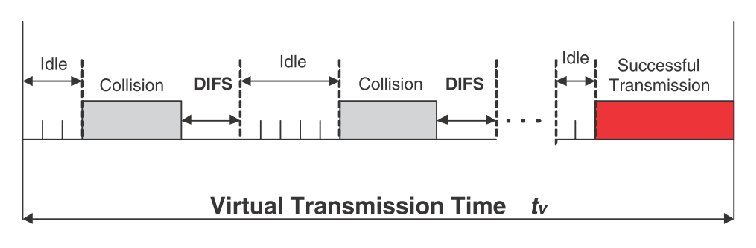
\includegraphics[width=9cm]{eps/80211dcf.eps}}
\caption{IEEE 802.11 DCF對實際傳輸時間的定義} \label{fig:80211dcf}
\vspace{-0.2cm}
\end{center}
\end{figure}
%-------------------

%-------------------
\begin{figure}[hbt]
\begin{center}
\centering {\includegraphics[width=9cm]{eps/sys_parameters.eps}}
\caption{系統參數表} \label{fig:sys_parameters}
\vspace{-0.2cm}
\end{center}
\end{figure}
%-------------------

然而,此分析模型是建立在「所有的工作站隨時隨地都可傳送封包」的前提上(在\cite{tn00_cali}中被稱作 asymptotic condition)。另外,在由幾何分布所構成的後退機制裡,直到每次資料傳輸成功之前用來表示通道使用情形的程序 (idle slots, collisions, successful transmissions)是「可再生」的,每次成功完成資料傳輸的當下在時間上被稱作「再生點」。該作者利用此特性定義第 $j$ 次實際傳輸時間(virtual transmission time)為第 $j$ 次與第 $j+1$ 次資料成功傳輸的時間間距。如圖(4.1)所示,閒置區段(idle period)指所有工作站都處於後退(backoff)階段以致於媒體當下情形為閒置的時段,而碰撞(collision)表示同時有兩個或更多工作站正在進行資料傳輸造成不同的封包發生碰撞的時段,以上兩者皆發生於成功傳輸(successful transmission)之前。 

令 $t_v$ 為實際傳輸時間的平均值,$I_i$ 與 $T_c$, $i$ 分別表示在一次實際傳輸時間之中的第 $i$ 次閒置時段的大小及第 $i$ 次碰撞時段的長度,根據\Fig{fig:sys_parameters}的系統參數,「協議效能」$\rho$ 為 $\rho = \frac{ \overline{m} }{t_v} $,其中 $t_v = E(N_c)*(E(T_c)+DIFS+SIFS+ACK) + (E(N_c)+1)*E(I) + E(S)$。

上式出現的 SIFS 及 ACK 是因為封包發生碰撞啟動重傳機制時須等候額外的時間所致,我們稱之 EIFS(Extended Inter-Frame Spacing),在 Cali's model 中假設封包發生碰撞後相應的工作站須等候 DIFS 時間,而在我們的模型中以 EIFS 取代之。 
而表示 single-cell 無線區域網路(WLAN)中 $E[N_c]$, $E[T_c]$及$E[I]$的方程式已在先前的研究成果中\cite{tn00_cali}被推導出。

為了延伸 Cali's model 到於多節點、多重速率的無線環境,我們做了下列更動: 
(1) 在最初的 p-persistent 模型中,決定嘗試傳送資料的機率(attempt probability, $p_a$)的參數僅有後退時間(backoff timer value),為了實現載波偵測對 $p_a$ 的影響,在我們所提出的分析模型中,考量了載波偵測等因素並重新定義了 $p_a$。 \\
(2) 在 p-persistent 模型中,碰撞的定義為:同一時間於 single-cell 範圍內出現二或多筆同步傳輸(simultaneous transmission),而在我們所提出的分析模型中,我們考量不同傳輸速率對訊號的接收造成的影響,即不同傳輸速率對應不同的 SINR 最低門檻(minimum SINR threshold),並進一步定義碰撞區域(collision zone, CZ)的概念。CZ 表示一個特定範圍,在這個範圍內只要有二或多組傳送端/接收端同時進行資料傳輸,即會干擾到其他節點的傳輸品質,甚至於發生碰撞。在\cite{tn00_cali}中,所有位於CZ中的節點被稱作active nodes,而碰撞機率的計算亦有所更動。 \\
(3) 在 p-persistent 模型中,所有資料傳輸皆使用單一傳輸速率,而在我們所提出的分析模型中則根據不同的 SINR 值來選定所使用的傳輸速率,一個無線電波收發器的訊號接收、解析效能可能因其使用的傳輸速率而異。 \\
(4) 由於 Cali’s model 是針對 single-cell 無線區域網路(WLAN)而設計的,因此並沒有考慮到空間重複利用率(spatial reuse)的問題。在我們所提出的分析模型中,可經由調節 $T_{cs}$ 來決定空間重複利用率,並控制並行傳輸(concurrent transmission)數量的多寡及訊號干擾的程度,藉此可進一步決定當下 SINR 值可負荷的最大資料傳輸速率,而最終的網路效能將由同步傳輸的數量及其使用的資料傳輸速率決定。 

另外,為了使上述於分析模型中更動的部分更加契合,我們假設網路環境符合下列情況: 
(A1) 分布於平面上的各節點符合 Poisson process,其節點密度(node density)為 $\lambda$。 \\
(A2) 所有節點隨時隨地都可傳送封包,即 asymptotic condition。 \\
(A3) 所有節點使用相同的功率 P 與訊號傳播模型如第 3 章所示,另外對一次使用傳輸速率 $r[i]$並成功的資料傳輸,其位於接收端的 SINR 值必須大於最低門檻(minimum SINR threshold)。 \\
(A4) 傳送端與接收端之間的距離須足夠靠近,以減少彼此對於同步傳輸(simultaneous transmission)、碰撞區域 (collision zone, CZ) 和 $d_{cs}$ 範圍外的並行傳輸(concurrent transmission)認知的差異。\\


\item [\bf ]{\textbf{\Kai C.1 資料傳輸嘗試機率(Attempt probability, $p_a$)的測定 }}\\
\vspace{-2mm}

資料的傳輸是否能成功進行取決於 $p_a$ 的大小,回顧前一段,在 asymptotic condition 之下,當一個節點試圖傳送封包時會先對媒體進行載波偵測,若此時媒體為閒置(idle)狀態則會啟動後退(backoff)機制並開始倒數計時,而 $p_a$ 之值受載波偵測、後退機制等因素影響。具體而言,一個傳送端進行資料傳輸必須符合以下三項條件(各自獨立):\\
(1) $E_1$ :$d_{cs}$ 範圍內無其他節點在傳送資料。 \\
(2) $E_2$ :由 $d_{cs}$ 範圍外的並行傳輸(concurrent transmission)造成的訊號干擾加總$I_{con,d_{cs},d_{pg}}$必須低於 $T_{cs}$ 。 \\
(3) $E_3$ :傳送端的後退計時器(backoff timer)倒數至 0。 
$p_a$傳送機率以方程式表示: $p_a = Pr\{E_1\} × Pr\{E_2\} × Pr\{E_3\} $

由 Poisson process,我們可以推論出: $Pr\{E_1\} = (1−p_a)^{\lambda \pi d_{cs}^2}$。同樣的,$Pr\{E_3\}$已於 Cali's model 中被導出: $Pr\{E_3\} = 2/(CW+1)$,CW 為平均競爭視窗(contention window)大小。 
另外,我們需要經由 $I_{con,d_{cs},d_{pg}}$ 來求得 $Pr\{E_2\}$之值,表示式為 $Pr\{E_2\} = Pr \{I_{con,d_{cs},d_{pg}} ≤ T_{cs}\}$。

我們令 $K = [ d_{pg} − d_{cs} / d_{cs} ] + 1$、一個傳送端的 $i_{th}$ tier 干擾節點為與其距離為 $i*d_{cs}$ 的節點,建立在 hexagon interference model 的架構下,估計整個範圍內約有 $min(6i, \lambda*(2\pi*i*d_{cs}^2 ))$ 個並行傳輸節點(concurrent transmitter)。上式第一項為考量空間重複利用率的因素,即先前提到的並行傳輸節點之間的距離至少須為 $d_{cs}$ ,而第二項指位於半徑 $i*d_{cs}$ 之內及 $(i+1)*d_{cs}$ 之外的平均節點數量。綜合上述資訊,我們可推得下式:
$$
I_{con,d_{cs},d_{pg}} =  \sum_{k=1}^K  \frac{GP*min \big\{6k,2k \lambda \pi d_{cs}^2\big\} }{ \big(k+1/2\big) ^\alpha  \big(d_{cs}\big) ^\alpha}
$$
值得注意的是, $I_{con,d_{cs},d_{pg}}$ 是一個以 $d_{cs}$ 為變數的方程式。因此當我們給定$d_{cs}$ ,即可求出其最終值,而 $Pr\{E_2\}$便成為一個二元判斷式(binary values with 0 or 1)。若給定的 $d_{cs}$對應的 $Pr\{E_2\}$為 0,則表示傳送端根據載波偵測相關的參數設定對當下環境的評估結果為:「誘因不足,若進行資料傳輸恐效果不彰。」,因此不會嘗試存取媒體以進行資料傳輸。 \\


\item [\bf ]{\textbf{\Kai C.2 資料傳輸速率(Data rate)的選定 }}\\
\vspace{-2mm}

根據 Shannon capacity theorem \cite{book2002_wc},在現有的載波偵測機制下能達到的最高資料傳輸速率 R 可表示為: $R = W*log_{2}(1+SINR)$。其中 W 為通道頻寬(單位 Hertz),另外,建立於 IEEE 802.11 架構下的網路支援的資料傳輸速率為不連續的,\Fig{fig:sinr_thre}為 IEEE802.11a 標準\cite{ieee802.11a}下各資料傳輸速率 $r[i]$ 與其所需的 SINR 最低門檻 $\beta[i]$ 的對應表。例:若求得的SINR值大於最低門檻$\beta$之最大值24.56 dB,則資料傳輸速率可設定為 54Mbps;反之,若 SINR 值小於 $\beta$ 之最小值 6.02 dB,則傳送端會因任何資料傳輸速率皆不適用而停止資料傳送。此外,透過觀察$r[i]$及$\beta[i]$數值的變化,我們發現適當的選擇各項參數似乎可增強對節點對訊號干擾的容忍度。若接收端的SINR 值與其選定的 $r[i]$ 所對應的 $\beta[i]$ 彼此之間有一定程度上的差距,則接收端可負荷部分因 $d_{cs}$ 範圍內的同步傳輸(simultaneous transmission)所造成的訊號干擾。 \\

%-------------------
\begin{figure}[hbt]
\begin{center}
\centering {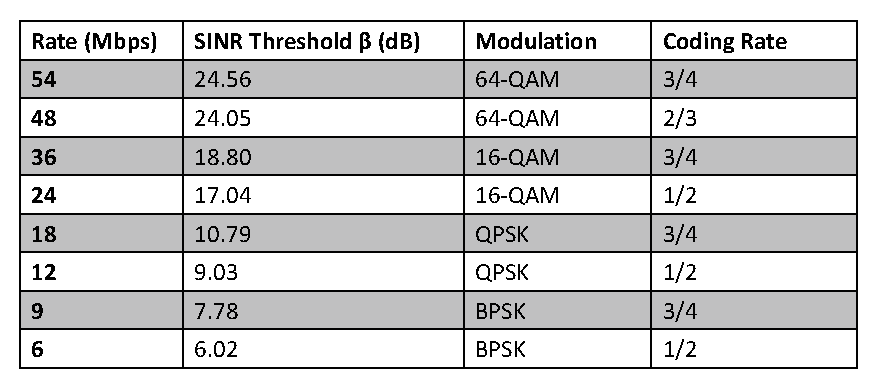
\includegraphics[width=9cm]{eps/sinr_thre.eps}}
\caption{IEEE 802.11a中各速率最低SINR需求} \label{fig:sinr_thre}
\vspace{-0.2cm}
\end{center}
\end{figure}
%-------------------

\item [\bf ]{\textbf{\Kai C.3 碰撞區域(Collision Zone, CZ)的定義  }}\\
\vspace{-2mm}

接收端的 SINR 值必須大於特定的最低門檻 $\beta[i]$才能負荷其對應的資料傳輸速率 r[i],若接收端的 SINR 值與其使用的 r[i]對應的 $\beta[i]$ 存在著一定程度上的差距,則可承受部分因 $d_{cs}$ 範圍內的同步傳輸所造成的訊號干擾,即 $d_{cs}$ 內的同步傳輸不一定會降低傳輸品質,此概念對於 CZ 的定義是必需的,在\cite{tn00_cali}中,所有位於 CZ 範圍內的節點被稱作 active nodes。 

%-------------------
\begin{figure}[hbt]
\begin{center}
\centering {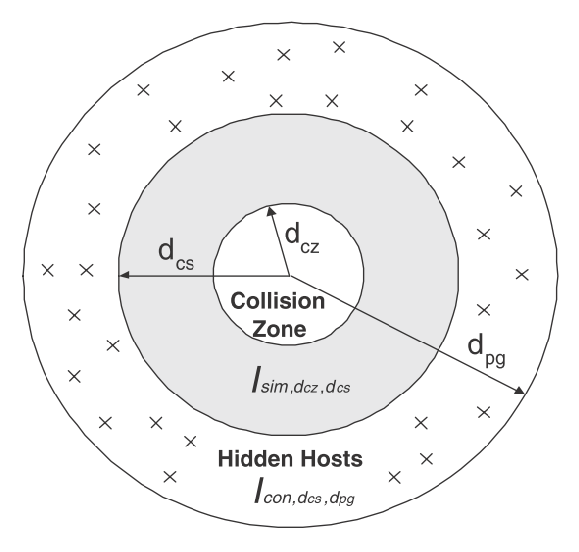
\includegraphics[width=8cm]{eps/czone.eps}}
\caption{碰撞區域(CZ)之示意圖} \label{fig:czone}
\vspace{-0.2cm}
\end{center}
\end{figure}
%-------------------

我們定義 CZ 為一半徑為 $d_{cz}$ 的圓形範圍(關於 $d_{cz}$ 之值本小節後半部將詳述之),在此範圍內若出現同步傳輸必定會導致碰撞的發生,載波偵測能避免 $d_{cs}$ 內的並行傳輸 (concurrent transmission) , 但無法避免 $d_{cs}$ 內的同步傳輸 (simultaneous transmission),因此我們令位於 $d_{cz}$ 外、$d_{cs}$ 內由同步傳輸所產生的訊號干擾的總和為 
$I_{sim,d_{cz},d_{cs}}$,表示除了 $I_{con,d_{cz},d_{pg}}$ 之外的訊號干擾。並進一步觀察目前使用的 r[i]所對應的 $\beta[i]$是否能負荷這些額外的訊號干擾。在圖(4.3)中,我們將陰影部分切割為 K 個「甜甜圈」形狀的區域,每個區域的「厚度」皆以 Δd = ($d_{cs}$ - $d_{cz}$ ) / K 表示,接著分別計算各個區域內由該區域的傳送端所產生的干擾總和,最後將所有求得的干擾數值予以加總,就可以得到同步傳輸所產生的訊號干擾的總和$I_{sim,d_{cz},d_{pg}}$ 。

我們必須確保當下的網路環境能夠負荷特定的傳輸速率 r[i],即所有位於 CZ 範圍外的干擾加上環境本身的雜訊不得踰越接收端訊號功率 $P_r = GP / D^{\alpha}$ 與 SINR 最低門檻$\beta[i]$的比值。
若 $GPD^{-\alpha} / { I_{sim,d_{cz},d_{pg}} +  \eta } $與 $\beta[i]$之間的差距大到足夠負荷由 $d_{cs}$ 範圍內的同步傳輸造成的干擾,則$d_{cz}$ 的範圍將會縮減。另外,由 CZ 的定義我們可得知,CZ 範圍內出現的任意同步傳輸將會導致碰撞的發生,因此我們令 CZ 內的 active node 數量為 H,即 $H =  \lambda \pi d_{cz}^2$。


\item [\bf ]{\textbf{\Kai C.4  網路效能(Network Capacity)的計算 }}\\
\vspace{-2mm}

我們以一個由 $E[N_c]$、$E[T_c]$、$E[I]$、$E[S]$和其他若干參數所構成的方程式,來描述實際傳輸時間 $t_v$ 。而 $E[N_c]$、$E[T_c]$、$E[I]$及$E[S]$也已依序以由 $p_a$、$H$ 等參數所組成的方程式表示,意即當我們在推導多節點、多重速率無線環境下的 $p_a$ 及 $H$ 時可進一步的推論出 $E[N_c]$、$E[T_c]$、$E[I]$及$E[S]$之值。

$E[T_c]$與$E[S]$之值取決於資料傳輸當下所使用的速率,我們令 $\gamma = 1/r[i]$,r[i]為前二小節所提到的對應 SINR 最低門檻 $\beta[i]$ 的資料傳輸速率,$E[S]$可以下列方程式表示: $E[S]=\gamma*m+SIFS+\gamma*ACK+DIFS$,而資料封包及 ACK 封包皆假設以特定傳輸速率 r[i]傳送。

如\cite{tn00_cali}所示,$E[T_c]$為所有發生碰撞的封包中最大的資料長度。而須考量的因素除了資料傳輸速率之外,先前所提到的 active nodes 亦須計算在內,其數量即為 CZ 內的節點數量。

同樣的,藉由定義 CZ 內的節點為 active nodes,我們可以將 $E[N_c]$ 用下列方程式表示。
$$
E(N_c) =  \frac{1-(1-p_a)^H}{Hp_a(1-p_a)^{H-1}} -1
$$

藉由用來決定 $d_{cs}$ 範圍內的媒體情形是否為閒置(Idle)的載波偵測機制,假設 $d_{cs}$ 內的節點總數為 $M$, $M = \lambda*\pi*d_{cs}^2$),我們可將預期的閒置時段 E[I] 定義為
$$
E(I) =  \frac{(1-p_a)^M*t_{slot}}{1-(1-p_a)^M}
$$


利用這些數學式,我們將可求得多節點、多重速率無線環境下的平均資料傳輸時間,也能夠求得載波偵測範圍內的「協議效能」。 

最後,令網路覆蓋範圍為 A、一個傳輸端的「使用區域」為 $A_s$ ,我們定義最終的網路效能 (network capacity) C 為並行傳輸(concurrent transmission)總數 $N_{tx}$ 與「協議效能」$\rho$ 的乘積,即$C = N_{tx}*\rho$。\\

\end{enumerate}

\subsubsection{第三年研究方法與執行進度}
\begin{enumerate}
\setlength\parindent{2em}

\item [\bf A.]{\textbf{\Kai 網路效能最佳化 }}\\

研究其他種最佳化演算法的原理與應用,並透過代入數據來驗證效能,實現前幾年提到:在變化快速的無線環境下,以最快的速度找出最佳$T_cs$以獲得最佳網路效能(network capacity)。

利用推導出的網路效能方程式,即$C = N_{tx}*\rho$,拆解後可以發現影響其數值大小的參數甚多。這裡主要討論的參數為 $d_{cs}$ 、$CW$及範圍內節點數目。其他參數如:節點分布範圍$A$、傳輸功率$P$、節點間最大距離$D$、通道衰減常數$\alpha$及訊號傳播範圍$d_{pg}$等皆假定為常數。訊號範圍內的節點個數將會影響最佳網路效能的$d_{cs}$與$CW$之值。在節點個數變動十分快速的情況之下(如廣場上正在使用行動上網的手機、平板、穿戴設備或其他可連網的行動裝置之數量),必須以最快的速度計算出當下能獲得最佳網路效能的$d_{cs}$及$CW$,很顯然漫無目的隨機選擇很沒有效率,我們將針對這個議題引入數種最佳化演算法:\\
(1) 登山演算法(Hill Climbing)\\
(2) 模擬退火法(Simulated Annealing) \\
(3) 基因演算法(Genetic Algorithm) \\
(4) 改良型演算法(Enhanced Algorithm)\\
以求在有限時間內達到找出能產生最佳網路效能的$d_{cs}$及$CW$值。\\

\item [\bf ]{\textbf{\Kai A.1. 登山演算法(Hill Climbing) }}\\

登山演算法之概念為:給定一個二維函數圖形,x軸選定任一點並計算y軸數值(在此x軸為$d_{cs}$、y軸為網路效能$C$),再隨機往左或右移動並計算數值。計算結果較佳則繼續前進,若計算結果較差則轉向換邊前進,直到求得峰值為止。

此方法的優勢為快速、穩定、架構簡單且容易實現。但存在著明顯的缺陷,即最終找到的最佳解絕大部分為區域最佳解(local optimal solution),而非我們所追求的全域最佳解(global optimum solution),因此常常發生所找到的$d_{cs}$所對應的網路效能(network capacity)並未有效而顯著的提高。\\


\item [\bf ]{\textbf{\Kai A.2. 模擬退火法(Simulated Annealing)  }}\\

模擬退火法是由登山演算法延伸而來,不同之處在於計算結果較差(下坡)時不會直接判定轉向,而是由一個機率式 $p_{con} = exp (- \Delta t / T)$ 來判斷繼續前進或是轉向。機率式的 $p_{con}$ 表示下坡繼續前進的機率、$\Delta t$為本次與前次計算結果差異之絕對值、$T$為剩餘時間(由預先設定的搜尋時間開始倒數至0為止)。由此式我們可以得知,$\Delta t$越大即「下坡」的幅度相對的越大,若套用到我們的分析模型表示目前所選定之$d_{cs}$會使網路效能大幅度降低,因此$p_{con}$也相對較低,即有很大的機率會轉向。另外若搜尋的時間持續太久,即$T$越接近0,亦會使$p_{con}$持續降低終致轉向,而停止搜尋條件為:(1)轉向2次;(2)$T$倒數至0。

相對於登山演算法,此方法較有機會找到全域最佳解,而非搜尋到峰值就停止。但仍有一些情況無法避免且會導致效率不彰,如圖(5.1)所示,為節點個數為20時的$d_{cs}$與網路效能C的分布情形,我們可以很明顯地看到當$d_{cs}$在50以下對應的C全部都為0。其原因如(4.9)式所述,由於干擾總和 $I_{con,d_{cs},d_{pg}}$ 高於$T_{cs}$以致使節點判定目前媒體為忙線(busy)而停止傳送封包。如果一開始選定的$d_{cs}$在0到50之間,有可能造成時間浪費在搜尋「0點」上而導致效率不彰。另外,若碰到「緩降坡」的情形,即連續下坡但因下降的幅度$\delta t$皆非常小而不會轉向搜尋,亦會造成時間的浪費。因此我們將會針對上述提到的問題對模擬退火法做些許的修改以使之更適用於我們所提出的分析模型。\\


\item [\bf ]{\textbf{\Kai A.3. 基因演算法(Genetic Algorithm)  }}\\

基因演算法的運作較類似於原始的不規則隨機搜尋,大致的概念為遺傳學中所述的「將優良的樣本相互交配有機會產生更優良的下一代」,其實際操作方法如下:\\
(1) 隨機選擇數組樣本($d_{cs}$)組成母體。\\
(2) 計算樣本的「適應函數」(fitness function, 在此為網路效能$C$)\\
(3) 挑選幾組適應函數佳($C$值較大者)的樣本進入下一階段。\\
(4) 進行「交配」(crossover),做法為將剩下的樣本($d_{cs}$)轉換為二進制並互相交換任意個位元(bit)。\\
(5) 進行「突變」(mutation),即各樣本隨機自行改變1~n個位元(n為最大位元數,例:01011110,其n = 8),亦可不做改變。\\
(6) 將所有樣本轉回十進制並重複(2)至(5)的動作直至適應函數之值達到預先設定的目標(在此不適用,因無法事先得知最佳解)或搜尋時間終了為止。\\

此方法的優勢在於最終搜尋到的解多為全域最佳解,不會像登山法及模擬退火法常受限於區域最佳解。由於登山法及模擬退火法皆為「單粒子」搜尋法,即搜尋過程中兩者皆從一個點出發,而基因演算法為「多粒子」搜尋法,在計算適應函數、交配(crossover)及突變(mutation)的過程中是多點($d_{cs}$)同步進行的,因此較不會發生上述所提到的「0點」問題。但計算過程較為繁瑣且耗時,效率較傳統最佳化演算法來的低。\\


\item [\bf ]{\textbf{\Kai A.4. 改良型演算法(Enhanced Algorithm) }}\\

上述提到的三項最佳化演算法皆對增進網路效能(network capacity, $C$)有幫助,但存在著各自的缺陷。登山演算法快速、穩定且容易操作,但運算結果易侷限於區域最佳解以及先前提到的「0點」問題;模擬退火法稍微改善了登山演算法的區域最佳解問題,但實際運作時其效果有限且「0點」問題仍然存在;基因演算法則是透過多點搜尋有效解決了「0點」問題,但較為費時、計算繁瑣且效率不佳。因此,在考量以上因素後,我們提出了一種改良型演算法(Enhanced Algorithm),結合上述提及的優點並加以改進。

在此我們對原始的模擬退火法做了一些適應性的改良:\\
(1) 起始搜尋點的選定:\\
  原始的模擬退火法是直接選定單一點開始搜尋,我們取基因演算法「多粒子」的特點,將x軸($d_{cs}$)劃分為多個區域,並在各個區域隨機取一個點計算C,並取C最高者為起始搜尋點,這樣不僅可以大大降低從0點開始搜尋的機率,亦可確保最後搜尋到的解(optimized network capacity)能保持一定程度上的品質。\\
(2) 記錄搜尋過的節點:\\
  我們新增一個參數$MaxC$來記錄目前搜尋過具有最大網路效能的$d_{cs}$值,並持續更新,另外以$S_{flag}$記錄起始搜尋點,如此遇到下坡轉向時可直接跳回起始點換邊搜尋,以及避免搜尋到重覆的點造成時間的浪費。\\
(3) 加速與跳點搜尋:\\
  此項是針對「緩降坡」及「緩升坡」情形,即下坡時$\delta t$持續很小因而不轉向與上坡時$C$增加的幅度持續很小,這些情形可能會造成時間的浪費且對尋找最佳值無益。因此我們令其持續下坡超過一定的次數時放棄繼續下坡並直接隨機跳至另一個$d_{cs}$值繼續搜尋,若跳躍後的$d_{cs}$值所對應的$C$較佳,則接下來將從該點繼續搜尋,反之將退回原點轉向搜尋。而持續上坡時增加其上坡的幅度,如此不僅可增加搜尋的效率,亦可減少時間的浪費,有助於在變化十分快速的無線環境之下更快速的找到能使網路效能最佳化的$d_{cs}$值。

另外,我們在以上演算法之中皆加入了調整競爭視窗($CW$)的機制。一般而言,$CW$值是一開始環境參數設定時所定,在搜尋過程中不會做修改,但由圖(5.1)我們可了解到$CW$值對網路效能$C$存在著一定程度的影響。而一開始所定的$CW$值並不一定為最適合當下環境的$CW$值,因此在找到最佳$d_{cs}$值而停止搜尋後,我們會針對不同的$CW$值再做網路效能$C$的計算,如此一來便能夠找到最佳$d_{cs}$、$CW$之組合以實現最佳化網路效能(network capacity)的目的。\\


\item [\bf B.]{\textbf{\Kai 理論值計算及分析 }}\\

針對上述提及的演算法,我們使用\Tab{tab:env-parameter}所示的環境參數,來比較上述四種演算法應用於此分析模型的效能,並觀察一個特定範圍的無線網路環境中各節點(可能為固定節點或移動節點)存取網路資源的情形。

%%%%%%%%%%%%%%%%%%%%%%%%%%%%%%%%%%%%%%%%%%%%%%%%%%%
% \Tab{tab:env-parameter}
\begin{table}[!htb]
\centering
\caption{環境參數設定值}
\vspace{0.2cm}
\small
\begin{tabular}{|c|c|}
\hline
Node = 10, 62, 200 & Area = 500*500 $m^2$ \\
\hline
Max distance between $T_x$ and $R_x$ = 50 m & Transmit power(fixed) = 0.85 mW \\
\hline
SIFS = 16 $\mu s$ & Slot time = 9 μs \\
\hline
DIFS = 34 $\mu s$ & Pass loss exponent = 4 \\
\hline
Propagation range = 302 m & Traffic load = 1125 Bytes$/$packet\\
\hline
Time limit = 300 sec & Search period per round = 10 sec\\
\hline
\end{tabular}
\label{tab:env-parameter}
\end{table}
%%%%%%%%%%%%%%%%%%%%%%%%%%%%%%%%%%

由於要計算出包含$d_{cs}$及$CW$等因素在內的所有情況,需耗費極為可觀的時間。在無線環境之下,節點數量的變化與移動是不斷的在變動且無法準確預測的,因而必須盡可能的在最快的時間內計算出符合當下情形,即能夠產出最大網路效能的$d_{cs}$值並套用於所有節點。我們針對上述所提到的四種演算法做數次的$d_{cs}$搜尋,每次搜尋時啟動一倒數計時器,發生逾時時,該次搜尋完成後停止並開始調整競爭視窗(contention window, $CW$),全部完成後觀察:\\
(1)是否曾經找到最佳$d_{cs}$位置? 若有找到最佳的$d_{cs}$位置,次數為何? 若沒有找到最佳的$d_{cs}$位置,目前所找到之最佳位置於何處? 其對應的網路效能$C$及與最佳位置所對應之網路效能$C_{opt}$的差距為何? \\
(2)各個演算法所定義的搜尋機制,在搜尋過程中是否確實有助於在有限時間內接近並找到最佳位置之所在? 其效率為何?

基於上述的分析模型,我們最後會將這些機制整理成完整的演算法,接著利用數學分析以及網路模擬器來分析與驗證,初步模擬環境如\Tab{tab:ns2-parameter}所示。
我們採用網路模擬器NS-2來模擬先前提到的情境,將各個最佳化演算法所搜尋到的$d_{cs}$及CW值代入分析,並求出其最終的網路效能(network capacity),以驗證演算法的效能是否符合理論。\\



%%%%%%%%%%%%%%%%%%%%%%%%%%%%%%%%%%%%%%%%%%%%%%%%%%%
% \Tab{tab:ns2-parameter}
\begin{table}[!htb]
\centering
\caption{Parameters used in NS-2 simulation}
\vspace{0.2cm}
\small
\begin{tabular}{|c|c|}
\hline
\multicolumn{2}{|c|}{\bf{Propagation model:Two-Ray Ground}}\\
\hline
\multicolumn{2}{|c|}{\bf{Channel type:WirelessChannel}}\\
\hline
\hline
Mac type:802.11Ext & Physical layer type:WirelessPhyExt \\
\hline
Slot time = 9 $\mu s$ & (Ommi-)Antenna gain = 1 \\
\hline
SIFS = 16 $\mu s$ & Fixed transmit power = 0.8 mW \\
\hline
DIFS = 34 $\mu s$ (2 Slot time + SIFS) & Simulation range = 500 x 500 ($m^2$) \\
\hline
\multirow{2}{*}{Path loss exponent = 4} & $CW_{min} = 8$\\
                                  &$CW_{max} = 1024$\\
\hline
Packet size = 1125 Bytes & RTSThreshold = 3000 (disabled)\\
\hline
\end{tabular}
\label{tab:ns2-parameter}
\end{table}
%%%%%%%%%%%%%%%%%%%%%%%%%%%%%%%%%%



\end{enumerate}


%\newpage
\subsection{預期成果}

在這份三年的計畫中,我們總結每一年的預期成果如下: 

\begin{enumerate}
\setlength\parindent{2em}
\item [\textbullet]	{\textbf{\Kai 第一年預期成果}}\\

% 12.3.1 第一年研究方法與執行進度
% A. 利用調節載波偵聽門檻 (T cs ) 實現空間多樣性
% B. 利用調節資料傳輸功率 (P tx ) 實現空間多樣性
% C. 其他相關研究
% D. 建立網路模型
在第一年的執行時間裡,預期會有下列初步研究成果。
為了分析$T_{cs}$與空間重複利用率之間的關係,我們將詳細研究相關的參考文獻,將透過估算及實驗結果來分析$T_{cs}$對於整體網路效能(network capacity)的影響。

針對不同的$T_{cs}$,藉由估算$d_{cs}$範圍外的干擾程度來設定其最適合的資料傳輸速率。在「$d_{cs}$範圍內的同步傳輸(simultaneous transmission)必定會產生碰撞」方面,可藉由給定適當的資料傳輸速率$r_i$,使接收端所收到的干擾訊號不超過$Pr/\beta[i]$,避免碰撞的發生。($Pr$:接收端收到的訊號強度;$\beta[i]$:對於資料傳輸速率$r_i$而言的,最低SINR門檻值)。
為了讓網卡傳輸功率受限的行動裝置實現降低訊號干擾與節能的目的,可以透過單通道無線環境的演算法,來決定當下的環境中各個節點適用的最小傳輸功率。透過對環境的適應並自動調節AP之間傳輸功率與速率,預期可以達成提升整體網路效能的目標。
根據接收到的SINR值,動態地決定每次資料傳輸所使用的傳輸速率,給定的資料傳輸速率仍需符合Shannon capacity的限制。並研究空間重複利用率與傳輸功率跟$T_{cs}$之間的關係,觀察調節傳輸功率和調節$T_{cs}$的所產生的效應為何。
關於$T_{cs}$、傳輸功率和其他MAC的相關參數對網路效能(network capacity)所產生的影響之研究,有相當多的切入點可以研究。我們會針對這方面的相關研究做一定程度的蒐集和統整,彙整這些作者們如何去適當的調節、運用這些參數。
然後研究以IEEE 802.11 Distributed Coordination Function (DCF)為基礎的多點跳躍、多重速率的無線網路環境,建立訊號傳播與干擾模型。探討資料傳輸的成功與否及可用的傳輸速率大小,與整體訊號干擾的程度之間的關係。\\

\item [\textbullet]	{\textbf{\Kai 第二年預期成果}}\\

% 探討演算法
% A. LMST-DCUA
% B. PCSadapt
% C. 網路效能方程式推導
% C.1 資料傳輸嘗試機率 (Attempt probability, p a ) 的測定
% C.2 資料傳輸速率 (Data rate) 的選定
% C.3 碰撞區域 (Collision Zone, CZ) 的定義
% C.4 網路效能 (Network Capacity) 的計算
第二年的進度規劃,我們預期去探討相關的研究並且分析網路效能方程式的各種參數。
利用Cali’s model 來更進一步的延伸至多節點、多重速率的無線網路,將最終的網路效能(network capacity)以一個由$d_{cs}$, SINR, $\beta[i]$及其他PHY/MAC相關的各項參數所組成的方程式表示。
並且研究相關的演算法,如LMST-DCUA、PCSadapt等。

前者LMST-DCUA全名為
結合傳輸功率選定(LMST)及$T_{cs}$調節(DCUA)的演算法。其中LMST為決定節點傳輸功率的演算法,其流程又分為資訊蒐集、拓樸(topology)建立及選定傳輸功率三個階段。在資料蒐集的階段,節點間藉由Hello message來交換彼此的資訊。接著以Prim’s algorithm建立包含鄰近節點資訊的最小成本擴張樹,最後再根據這些資訊來決定傳輸功率之值。而DCUA全名為Distributed carrier sense update algorithm,其概念在於觀察資料傳輸過程中發生碰撞的頻率來調整載波偵聽門檻。

後者PCSadapt全名為
PCS Adaptation Algorithm Based on Loss Differentiation,是為一個結合傳輸速率選定與$T_{cs}$調節的演算法。它將整個資料傳輸的流程分為 (1) adaptation (2) normal operation兩個階段。處於階段(1)時,會進行傳輸速率的選定,環境中所有節點各自將其最小競爭視窗(CWmin)設定為一較大的值,以避免碰撞頻繁發生,透過蒐集各節點的RSSI (Received Signal Strength Indicator,一個類似SINR、用來衡量接收端訊號強度的基準,單位為功率),RSSI值小表示干擾或訊號衰減程度大,選擇低傳輸速率較為合適,相對的RSSI值大表示該節點可負荷較高的傳輸速率。
在網路效能方程式裡面,我們將分析這項參數。如:資料的傳輸是否能成功進行取決於$p_a$(資料傳輸嘗試機率,Attempt probability)的大小;根據SINR資訊來挑選資料傳輸速率 (Data rate);定義碰撞區域(Collision Zone, CZ),在此範圍內若出現同步傳輸必定會導致碰撞的發生,雖然載波偵測能避免$d_{cs}$內的並行傳輸(concurrent transmission),但無法避免$d_{cs}$內的同步傳輸(simultaneous transmission)。分析完相關參數後,再去計算整體網路的效能(Capacity)。\\

\item [\textbullet]	{\textbf{\Kai 第三年預期成果}}\\

% A. 網路效能最佳化
% A.1. 登山演算法 (Hill Climbing)
% A.2. 模擬退火法 (Simulated Annealing)
% A.3. 基因演算法 (Genetic Algorithm)
% A.4. 改良型演算法 (Enhanced Algorithm)
% B. 理論值計算及分析
基於前兩年的計畫成果,我們可以得到網路的效能方程式,接下來會去尋找有效率的最佳化演算法讓整體網路的表現提升到最佳狀態。並且分析相關的演算法,結合其優點,設計出適用於這個網路環境的演算法,透過代入數據以驗證其效能,實現先前提到的在變化快速的無線環境下以最快的速度找出最佳$T_{cs}$以獲得最佳網路效能(network capacity)的目的。
最後使用網路模擬器來模擬先前所描述的情境,將各個最佳化演算法得到的網路參數代入分析,並求出其最終的網路效能(network capacity),以驗證演算法的效能是否符合理論。
我們將研究各種不同的網路環境與拓樸,在這些規律與變動的網路環境中,藉由演算法去調整網路參數,使整體效能提高。經由實驗模擬,我們預期所提出的演算法能夠有效率的提升網路效能。\\


\end{enumerate}
\end{description}

\newpage
\begin{thebibliography}{00}

\bibitem{ieee802.11a} IEEE 802.11a WG Part 11: Wireless LAN Medium Access Control (MAC) and Physical Layer (PHY) Specifications: High-speed Physical Layer in the 5 GHz Band, 1999.
\bibitem{acm2005_smcwd} A. Akella, G. Judd, P. Steenkiste, and S. Seshan, “Self Management in Chaotic Wireless Deployments”, In Proc. ACM MobiCom, pp. 185-199, Aug. 2005.
\bibitem{ccr2004_rws} P. Bahl, A. Adya, J. Padhye, and A. Wolman, “Reconsidering Wireless Systems with Multiple Radios”, ACM SIGCOMM Computer Communications Revie`w (CCR), 34(5):39-46, Oct. 2004.
\bibitem{mobicom04_ssch} P. Bahl, R. Chandra, and J. Dunagan, “SSCH: Slotted Seeded Channel Hopping for Capacity Improvement in IEEE 802.11 Ad-hoc Wireless Networks”, In Proc. ACM Int’l Conference Mobile Computing and Networking (MobiCom), pp. 216-230, Sep. 2004.
\bibitem{mobihoc04_tc} M. Burkhart, P. von Rickenbach, R. Wattenhofer, and A. Zollinger, “Does Topology Control Reduce Interference ?”, In Proc. ACM MobiHoc, pp. 9-19, May 2004.
\bibitem{tn00_cali} F. Cali, M. Conti, and E. Gregori, “Dynamic Tuning of the IEEE 802.11 Protocol to Achieve a Theoretical Throughput Limit”, IEEE/ACM Transactions on Networking, 8(6):785-799, Dec. 2000.
\bibitem{vtc03_sr} X. Guo, S. Roy, and W. S. Conner, “Spatial Reuse in Wireless Ad-hoc Networks”, In Proc. IEEE VTC, pp. 1437-1442, Oct. 2003.
\bibitem{mobicom01_ramp} G. Holland, N. Vaidya, and P. Bahl, “A Rate-adaptive MAC Protocol for Multi-hop Wireless Networks”, In Proc. ACM/IEEE MobiCom, pp. 236-251, Jul. 2001.
\bibitem{sigcomm05_rwpcs} K. Jamieson, B. Hull, A. Miu, and H. Balakrishnan, “Understanding the Real-world Performance of Carrier Sense”, In Proc. ACM SIGCOMM, pp. 52-57, Aug. 2005.

\bibitem{mobicom06_kim} T.-S. Kim, H. Lim, and J. C. Hou, “Improving Spatial Reuse Through Tuning Transmit Power, Carrier Sense Threshold, and Data Rate in Multihop Wireless Networks”, In Proc. of ACM MobiCom, pp. 366-377, Sep. 2006.
\bibitem{tvt1986_cmrs} W. C. Y. Lee, “Elements of Cellular Mobile Radio Systems”, IEEE Transactions on Vehicular Technology, 35(2):48-56, May 1986.
\bibitem{twc05_hou} N. Li, J. C. Hou, and L. Sha, “Design and Analysis of an MST-based Distributed Topology Control Algorithm for Wireless Ad-hoc Networks”, IEEE Transactions on Wireless Communications, 4(3):1195-1207, May 2005.
\bibitem{mobihoc04_pcwn} A. Muqattash and M. Krunz, “A Single-channel Solution for Transmission Power Control in Wireless Ad Hoc Networks”, In Proc. ACM MobiHoc, pp. 210-221, May 2004.
\bibitem{infocom00_tcmwn} R. Ramanathan and R. Rosales-Hain, “Topology Control of Multihop Wireless Networks Using Transmit Power Adjustment”, In Proc. IEEE INFOCOM, pp. 404-413,  Mar. 2000.
\bibitem{book2002_wc} T. S. Rappaport, “Wireless Communications: Principles and Practice (Second Edition)”, Upper Saddle River Prentice-Hall, 2002.
\bibitem{mobihoc04_mcmac} J. So and N. Vaidya, “Multi-channel MAC for Ad Hoc Networks: Handling Multi-channel Hidden Terminals Using A Single Transceiver”, In Proc. ACM MobiHoc, pp. 222-233, May 2004.
\bibitem{infocom05_yang} X. Yang and N. Vaidya, “On Physical Carrier Sensing in Wireless Ad Hoc Networks” In Proc. IEEE INFOCOM, pp. 13-17, Mar. 2005.
\bibitem{infocom06_zhai} H. Zhai and Y. Fang, “Physical Carrier Sensing and Spatial Reuse in Multirate and Multihop Wireless Ad Hoc Networks”, In Proc. IEEE INFOCOM, pp. 1-12, Apr. 2006.


\bibitem{icc04_zhu} J. Zhu, X. Guo, L. L. Yang, and W. S. Conner, “Leveraging Spatial Reuse in 802.11 Mesh Networks with Enhanced Physical Carrier Sensing”, In Proc. IEEE Int’l Conference Communications (ICC), pp. 4004-4011, Jun. 2004.
\bibitem{infocom08_zeng} Z. Zeng, Y. Yang, and J. Hou, “How Physical Carrier Sense Affects System Throughput in IEEE 802.11 Wireless Networks”, In Proc. IEEE INFOCOM, Alaska, USA, pp. 13-18, Apr. 2008.
\bibitem{adhoc11_park} K. Park, J. Choi, J. Hou, Y. Hu and H. Lim, “Optimal Physical Carrier Sense in Wireless Networks”, Elsevier Ad Hoc Networks, 9(1):16-27, Jan. 2011.
\bibitem{tmc08_hou} T.-S. Kim, H. Lim and J. C. Hou, “Understanding and Improving the Spatial Reuse in Multihop Wireless Networks”, IEEE Transactions on Mobile Computing, 7(10):1200-1212, Oct. 2008.
\bibitem{cst14_survey} C. Thorpe and L. Murphy, “A Survey of Adaptive Carrier Sensing Mechanisms for IEEE 802.11 Wireless Networks”, IEEE Communications Surveys \& Tutorials, 16(3):1266-1291, Mar. 2014.
\bibitem{cccn08_phycs} Y. Z. Liu, X. M. Zhang, Q. Liu, and S. F. Dai, “Interference-aware Physical Carrier Sensing for Maximum Throughput in Ad Hoc Networks”, In Proc. Int’l Conference on Communications and Networking in China, pp. 60-64, Aug. 2008.
\bibitem{tvt09_power} B. Alawieh, C. M. Assi, and H. Mouftah, “Investigating the Performance of Power-aware IEEE 802.11 in Multi-hop Wireless Networks”, IEEE Transactions on Vehicular Technology, 58(1):287-300, Jan. 2009.
\bibitem{infocom07_interplay} T.-Y. Lin and J. C. Hou, “Interplay of Spatial Reuse and SINR-determined Data Rates in CSMA/CA-based, Multi-hop, Multi-rate Wireless Networks”, In Proc. IEEE INFOCOM, pp. 803-811, May 2007.
\bibitem{tmc09_aphycs} K.-J. Park, L. Y. Kim, and J. C. Hou, “Adaptive Physical Carrier Sense in Topology-controlled Wireless Networks”, IEEE Transactions Mobile Computing, 9(1):87-97, Jan. 2009.


\bibitem{ton09_optwmn} H. Ma, R. Vijayakumar, S. Roy, and J. Zhu, “Optimizing 802.11 Wireless Mesh Networks Based on Physical Carrier Sensing”, IEEE/ACM Transactions on Networking, 17(5):1550-1562, Oct. 2009.
\bibitem{infocom07_optcs} Y. Zhu, Q. Zhang, Z. Niu, and J. Zhu, “On Optimal Physical Carrier Sensing:Theoretical Analysis and Protocol Design”, In Proc. IEEE INFOCOM, pp. 2351-2355,  May 2007.
\bibitem{icl13_iter} D. Kim and S. Kim, "An Iterative Algorithm for Optimal Carrier Sensing Threshold in Random CSMA/CA Wireless Networks", IEEE Communications Letters, 17(11):2076-2079, Nov. 2013.

\end{thebibliography}
\label{LastPage}


\end{document}